% ----------------------------------------------------------------------------
% Projektbericht
% ----------------------------------------------------------------------------
\documentclass[12pt]{report}

% =======================================================
\newcommand{\MyName}{Niklas Deworetzki}
\newcommand{\MyTitle}{CS5341~--~Kernel-Architekturen in Programmiersprachen}
\newcommand{\MyTopic}{STG~--~Kernelsprache und Ausführungsmodell für nicht-strikte funktionale Programmiersprachen}        % Thema (Unterüberschrift)
% =======================================================

\usepackage[english, ngerman]{babel} % Automatische Worttrennung
\usepackage[babel]{csquotes}         % Anführungszeichen

\usepackage[T1]{fontenc}             % Umlaute und Sonderzeichen
\usepackage[utf8]{inputenc}          % für Eingabe und Ausgabe
\usepackage{scrhack}                 % unterdrückt Fehlermeldung von listings
\usepackage{parskip}

\usepackage{amsmath}                 % Mathematik
\usepackage{amssymb}                 % Mathematische Symbole
\usepackage{graphicx}                % Grafiken
\graphicspath{{images/}}             % Bilder werden aus images geladen
\usepackage{multicol}                % Mehrteilige Seiten

% Formatierungen für Grafiken und Elemente.
\usepackage[export]{adjustbox}
\usepackage[a4paper]{geometry}
\usepackage[titles,subfigure]{tocloft}
\usepackage{float}

% Formatierungen für Text, Überschriften, Inhaltsverzeichnis, etc.
\usepackage{fancyhdr}
\usepackage[nottoc]{tocbibind}
\usepackage{blindtext}
\usepackage{helvet}
\usepackage[lighttt]{lmodern}

\usepackage[pdftex,
pdfauthor={\MyName{}},
pdftitle={\MyTitle{}~--~\MyTopic{}}]{hyperref}

% BibLatex configuration
\usepackage[backend=bibtex]{biblatex}
\usepackage[toc,acronyms]{glossaries}
\bibliography{bibliography.bib}     % Pfad zur Datei, die Referenzen enthält

% Verschiedene Grafiken, Figuren, Listings
\usepackage[table]{xcolor} % Definiere eigene Farben
\usepackage{textcomp}      % Sonderzeichen (für Operatoren in Code, z.B.)
\usepackage{subfigure}     % Teilfiguren
\usepackage{filecontents}  % Lade Dateien (für Codebeispiele)
\usepackage{listingsutf8}  % Codeblöcke mit UTF-8 (Umlaute)
\usepackage{lstautogobble} % Entfernt führende Leerzeichen in Codeblöcken
% lstautogobble=false zum deaktivieren für einzelne Codeblöcke

% Grafikbibliothek zum Erstellen eigener Diagramme
\usepackage{tikz}
\usetikzlibrary{decorations.pathreplacing,shapes,arrows,positioning}


%------------------------------------------------------------------------------
% THM Farbdefinitionen
\definecolor{cdmain1}{RGB}{128, 186, 36}
\definecolor{cdmain2}{RGB}{74, 92, 102}
\definecolor{cdhighlight1}{RGB}{156, 19, 46}
\definecolor{cdhighlight2}{RGB}{244, 170, 0}
\definecolor{cdhighlight3}{RGB}{0, 184, 228}
\definecolor{cdhighlight4}{RGB}{0, 40, 120}
%------------------------------------------------------------------------------
\colorlet{fontcolor}{cdmain2}
\colorlet{headercolor}{cdmain1}
%------------------------------------------------------------------------------
% Schrift für Fußnoten
\renewcommand{\footnotesize}{\fontsize{10pt}{12pt}\selectfont}
%------------------------------------------------------------------------------
% Format für Tabellen
\newcommand\HeaderCell[1]{%
  \multicolumn{1}{c}{\cellcolor{cdmain2}\textcolor{white}{#1}}
}
%------------------------------------------------------------------------------

\lstdefinestyle{codestyle}{
  commentstyle=\itshape,
  keywordstyle=\bfseries,
  basicstyle=\ttfamily\small,
  breakatwhitespace=false,
  breaklines=true,
  keepspaces=true,
  showspaces=false,
  showstringspaces=false,
  showtabs=false,
  tabsize=2,
  frame=none,
  aboveskip=1em,
  belowskip=1em
}
\lstset{style=codestyle}

% ------------------------------------------------------------------------------
\makeatletter
\def\@makechapterhead#1{%
  \vspace*{50\p@}%
  {\parindent \z@ \raggedright \normalfont
    \interlinepenalty\@M
    \Huge\bfseries  \thechapter\quad #1\par\nobreak
    \vskip 40\p@
}}
\makeatother
\renewcommand*\cftchapnumwidth{2em}
\renewcommand*\cftsecnumwidth{3em}
%------------------------------------------------------------------------------
\makeglossaries{}
\makeatletter
\newcommand \Dotfill {\leavevmode \cleaders \hb@xt@ .8em{\hss .\hss }\hfill \kern \z@}
\makeatother
\renewcommand*\glspostdescription{\Dotfill}

\newacronym{stg}{STG}{Spineless Tagless G-Machine}
\newacronym{jvm}{JVM}{Java Virtual Machine}
\newacronym{cil}{CIL}{Common Language Infrastructure}
\newacronym{ram}{RAM}{Random Access Machine}
\newacronym{whnf}{WHNF}{Weak Head Normal Form}

%%% Local Variables:
%%% mode: latex
%%% TeX-master: "Ausarbeitung"
%%% End:

%------------------------------------------------------------------------------
% Redefine the fancy page style
%\fancypagestyle{fancy}{
\fancyhf{}
\fancyhead[R]{\thepage}
%\fancyfoot{}
\renewcommand{\headrulewidth}{0pt}
%}

\setlength{\headheight}{20mm}

% Redefine the plain page style
\fancypagestyle{plain}{%
  \fancyhf{}%
  \fancyhead[R]{\thepage}%
  \renewcommand{\headrulewidth}{0pt}% Line at the header invisible
  \renewcommand{\footrulewidth}{0pt}% Line at the footer visible
}

% ------------------------------------------------------------------------------


%------------------------------------------------------------------------------
% Zeilenumbrüche bei Unterstrichen (in langen Variablennamen)
\renewcommand\_{\textunderscore\allowbreak}

\newcommand\cn[1]{\textcolor{red}{\textsuperscript{[citation needed]}}}
% ------------------------------------------------------------------------------



% Offizielles Farbschema für Schrift verwenden:
% \color{fontcolor} % Macht Schrift blass


%==============================================================================
\begin{document}
% front matter
\pagestyle{empty}
%\newgeometry{left=40mm,right=15mm,top=30mm,bottom=20mm}
\pagenumbering{Roman}


\begin{titlepage}
  \begin{center}
    \begin{figure}
      % THM Logo
      \includegraphics[width=.9\textwidth]{LOGO_THM_CG_FB06}
    \end{figure}
  \end{center}
  % Title
  \Large
  \begin{center}
    \vspace{1cm}
    \textbf{\MyTitle{}}\linebreak
    \vspace{1cm}
  \end{center}
  \large
  Thema:\\
  \textbf{\MyTopic{}}

  \normalsize
  \vfill
  % \begin{tabular*}{\textwidth}[t]{l,c,l}
  \begin{center}
    \begin{tabular*}{0.75\textwidth}%
      {@{\extracolsep{\fill}}ll}

      {Vorgelegt von:} & {\MyName{}}\\
      {Matrikelnummer} & {5185551}\\
      {} & {}\\
      {} & {}\\
      {Eingereicht bei} & {}\\
      {Hochschulbetreuer/-in:} & {Prof.\ Dr.-Ing.\ Dominikus\ Herzberg}\\
      {} & {}\\
      {} & {}\\
      {Eingereicht am:} & {\today}

    \end{tabular*}
  \end{center}

  \vfill
\end{titlepage}
%==============================================================================

\addtocounter{page}{1}
\pagestyle{fancy}

\tableofcontents

\newcounter{savepage}
\setcounter{savepage}{\number\value{page}}
\newpage

%==============================================================================

% main matter
\pagenumbering{arabic}



\chapter{Einleitung}

Diese Ausarbeitung ist Teil der Dokumentation eines Projektes aus dem Modul \textit{CS5341~--~Kernel-Architekturen in Programmiersprachen}, welches im Wintersemester 2021/2022 stattfand.

Wie der Name es bereits verrät, liegt der Fokus der Veranstaltung auf Programmiersprachen mit einem kleinen Sprachkern, sogenannten \textit{Kernel-Sprachen}.
Diese Sprachen besitzen zumeist die Möglichkeit, sich mit eigenen Mitteln selbst zu erweitern, um so Schicht für Schicht höhere Abstraktionen aufzubauen, ohne diese explizit bei der Implementierung der Sprache zu unterstützen.
Das macht diese Sprachen nicht nur bei der Implementierung interessant, da die Implementierung eines kleinen Sprachkerns nur mit vergleichsweise geringem Aufwand verbunden ist.
Auch für Anwender sind solche Sprachen interessant, da sie zumeist flexibel sind, über Bibliotheken einfach erweitert werden können und die geringe Zahl der Kernfeatures ein schnelles Erlernen fördert.
Bekannte Vertreter für Kernelsprachen sind die verschiedenen Lisp-Dialekte, welche im Sprachkern lediglich Listen, Funktionen und Funktionsanwendungen bieten, während die restliche Funktionalität über Makromechanismen oder reflexive Programmierung entstehen.
Funktionale Sprachen wie Haskell oder Scala wandeln Quellprogramme mit komplexeren Bestandteil in eine kalkülartige Kernsprache um, welche für Analysen im Compiler und die Ausführung herangezogen wird.
Bei den objektorientierten Programmiersprachen ist Smalltalk als wichtiger Vertreter zu nennen.
Hier werden alle Sprachkonstrukte als Objekte dargestellt, welche sich Nachrichten senden können.

Während in den seminaristischen Vorlesungsstunden der Veranstaltung der Fokus zumeist auf den Mechanismen liegt, die in solchen Programmiersprachen verwendet werden, liegt der Fokus dieses Projektes in der Auseinandersetzung mit einem Programmiersprachenkern und besonders auf dem Ausführungsmodell, das diesem zugrunde liegt.
Die sogenannte \textit{STG-Sprache} wird verwendet, um eine Ausführungsumgebung für Haskell bereitzustellen, weswegen die Sprache nicht auf hoher Flexibilität und Erweiterbarkeit sondern vielmehr auf Maschinennähe und Kontrolle der ausgeführten Operationen zur Laufzeit basiert.
Die Besonderheiten dieser Programmiersprache wurden im Rahmen des Projektes untersucht und eine Implementierung der dazugehörigen Maschine in der imperativen Programmiersprache Java erstellt.

Diese Ausarbeitung ist in vier weitere Teile gegliedert, welche die verschiedenen Abschnitte des Projektes widerspiegeln.

\begin{itemize}
\item Kapitel~\ref{chap:grundlagen} befasst sich mit den Grundlagen hinter der STG-Sprache und der dazugehörigen Maschine.

\item Kapitel~\ref{chap:stg} beschreibt die für die Sprache definierten Sprachkonstrukte und deren Bedeutung zur Ausführungszeit.

\item Kapitel~\ref{chap:implementierung} assoziiert die einzelnen Sprachkonstrukte mit der zugehörigen Semantik sowie der Implementierung dieser für eine virtuelle Maschine in Java.

\item Kapitel~\ref{chap:ergebnisse} fasst die Ergebnisse des Projektes zusammen und reflektiert diese.

\end{itemize}


%%% Local Variables:
%%% mode: latex
%%% TeX-master: "../Ausarbeitung"
%%% End:


\chapter{Grundlagen}\label{chap:grundlagen}

Die \gls{stg} beschreibt eine abstrakte Maschine, sowie eine kleine Programmiersprache zur Programmierung ebendieser Maschine, die als STG-Sprache bezeichnet wird~\cite{Jones_StockHardwareSTG}.
Der vorwiegende Verwendungszweck liegt dabei in der Übersetzung und Ausführung von nicht-strikten funktionalen Programmiersprachen.
In solchen Programmiersprachen werden Ausdrücke verzögert und nur bei Bedarf ausgewertet.
Man spricht auch von der sogenannten \textit{Bedarfsauswertung} oder aus dem Englischen \textit{lazy Evaluation}.

% Closure

Dieser Ausführungsmodus kommt mit einer Reihe an großen Herausforderungen.
Zur Laufzeit muss zwischen ausstehenden oder unterbrochenen Auswertungen (sogenannten \textit{Thunks}) und bereits berechneten Werten unterschieden werden.
Gleichzeitig soll überflüssige Arbeit vermieden werden, indem Ausdrücke nur so oft wie nötig ausgewertet werden, um anschließend deren Wert für den Falle erneuter Auswertung zu speichern.
Zudem ist es in funktionalen Sprachen häufig der Fall, dass Ausdrücke nicht nur einfache Werte sondern auch Funktionen berechnen, wofür sogenannte \textit{Closures} verwendet werden, die Funktionsimplementierung und die für die Funktion sichtbaren Variablen Speichern.
Selbstverständlich soll eine Ausführungsumgebung, die all diese Anforderungen unterstützt, auch noch möglichst effizient sein und mit möglichst wenig Speicherbedarf und Rechenzeit auskommen.

Die STG-Maschine verspricht, als abstrakte Maschine diesen Anforderungen nachzukommen und wird seit den 1990er Jahren als wesentlicher Bestandteil in der Implementierung und Übersetzung von Haskell verwendet~\cite{Bolingbroke_WhatIsSTG}.
Im Ergebnis ist Performance von übersetzten Haskell Programmen häufig vergleichbar mit C~\cite{PeytonJones_FastCurry}.


\section{Graphenreduktion als Ausführungsmodell}

Die Verwendung einer abstrakten Maschine zur Ausführung einer Programmiersprache ist keine Besonderheit.
Die ursprünglich für Java entwickelte \gls{jvm} beschreibt eine abstrakte Stackmaschine, die entweder im Rahmen einer virtuellen Maschinenimplementierung ausgeführt wird, oder deren Semantik in Maschinencode für eine reale Maschine übersetzt wird~\cite{JVM17}.
Um die .NET Plattform herum entstand die \gls{cli}, welche standardisiert eine objektorientierte abstrakte Stackmaschine beschreibt.
In beiden Fällen soll die Verwendung einer abstrakten Maschine über die Tatsächliche Ausführungsumgebung abstrahieren, um so Programme plattform- und hardwareunabhängig ausführen zu können~\cite{Miller_CommonLanguageInfrastructure}.
Eine ähnliche Architektur bietet LLVM mit einer abstrakten Registermaschine~\cite{LLVM}.
Hier liegt der Fokus jedoch auf der Optimierung und Übersetzung von Programmen für diese abstrakte Maschine in realen Maschinencode.

All diese Modelle sind nah an dem Modell der handelsüblichen Computer, welche auch als sogenannte Sequentielle Maschinen Einzug in die theoretische Welt der Berechenbarkeit gehalten haben~\cite{Slot_ProblemSpaceInvariance}.
Die Grundannahmen sind hier, dass Rechenschritte einzelne gleichwertige Instruktionen darstellen, die nacheinander ausgeführt werden und jeweils eine Menge an Registern oder Speicherzellen beeinflussen können.

Die STG-Maschine wählt hier einen anderen Ansatz, der näher am Berechnungsvorgehen des Lambda-Kalküls ist:
Hier liegt das Programm als Datenstruktur vor, in der Ausdrücke als Knoten mit Kanten zu den verwendeten Teilausdrücken vorkommen.
Reduktionsregeln geben vor, wie schrittweise diese Datenstruktur reduziert werden kann, bis der Ausdruck schließlich eine sogenannte Normalform erreicht~--~eine einheitliche Form des Ausdrucks, die dessen ausgewerteten Wert repräsentiert.

Der Teil \textit{G-Maschine} der STG-Maschine steht dabei für \textit{Graphenreduktionsmaschine}.
Das auszuwertende Programm liegt also als Graph vor, der schrittweise reduziert wird~\cite{Wadsworth_RelationComputationalDenotational}.
Die Darstellung als Graph ermöglicht dabei eine genauere Beschreibung der Laufzeitsemantik eines Programmes, als es durch einen Baum möglich ist.
Darum wird diese Darstellung der klassischen Repräsentation als Syntaxbaum vorgezogen.
Abbildung~\ref{fig:graph-reduction} zeigt beispielhaft einen solchen Graphen für den Ausdruck $\mathtt{let}\ x\ =\ \frac{2}{y}\ \mathtt{in}\ x + x$.
Die Darstellung als Graph verdeutlicht hier, dass die beiden Vorkommnisse von $x$ auf denselben Wert verweisen.
Wird nun für $y$ der Wert $1$ bekannt, können nacheinander Reduktionsregeln angewandt werden, um den Graphen wie in Abbildung~\ref{fig:graph-reduction} auf einen einzelnen atomaren Wert zu reduzieren.

\begin{figure}
  \centering
  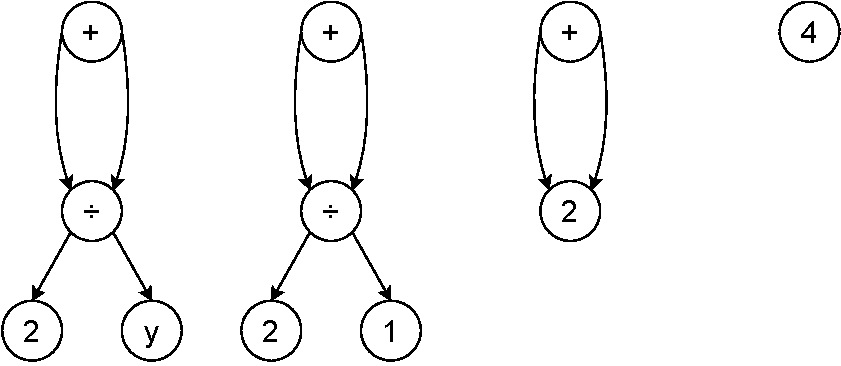
\includegraphics{graph-reduction}
  \caption[Schrittweise Reduktion eines Ausdrucks]{Schrittweise Redutkion des Ausdrucks $\mathtt{let}\ x\ =\ \frac{2}{y}\ \mathtt{in}\ x + x$}\label{fig:graph-reduction}
\end{figure}


\section{Besonderheiten der STG}

Die STG-Maschine definiert einige Erweiterungen für dieses Modell der Graphenreduktion.
Mit Hilfe dieser wird lazy Evaluation möglich und die effiziente Ausführung auf gewöhnlicher Hardware unterstützt.

Während die Darstellung eines Programms und dessen Ausdrücke als Knoten in einem Graph über die verschiedenen Ausprägungen der Laufzeitwerte abstrahiert und so im grundlegenden Modell die Unterscheidung zwischen Thunks, Werten und Closures für anonyme Funktionen überflüssig macht, müssen die durchgeführten Reduktionsregeln weiter eingeschränkt werden, um lazy Evaluation zu ermöglichen.
Dem Ansatz aus Abbildung~\ref{fig:graph-reduction} entsprechend würde der gesamte Graph reduziert, was der Idee der lazy Evaluation widerspricht.

Die Lösung ist hier das Definieren einer Normalform, welche die ausgewertete Form eines Ausdrucks darstellt.
Die Anwendung von Reduktionsregeln auf einen Teilgraphen in Normalform verändert diesen nicht mehr; ein Ende der Auswertung wurde erreicht.
Im Rahmen der \gls{stg} wird die \gls{whnf} verwendet~\cite{Wiki_Haskell}.
Die \gls{whnf} beschreibt, dass lediglich der Kopf eines Graphen in Normalform vorliegen muss, um ihn als ausgewertet zu betrachten.
Dies ist der Fall, wenn der oberste Knoten des Graphen einen Konstruktor oder eine eingebaute Funktionsanwendung beschreibt.
Der Rest des Graphen darf dabei unausgewertet vorliegen, wodurch die \gls{whnf} zu einer schwachen Normalform wird.
Am konkreten Beispiel einer verketteten Liste bedeutet dies, dass lediglich bekannt sein muss, ob der Kopf der Liste den Listenkonstruktor oder die leere Liste darstellt.
Ob die Liste abgesehen vom Kopf weitere Elemente enthält, wie lang diese Liste ist, oder wie das oberste Listenelement aussieht, ist dabei für die \gls{whnf} irrelevant.

Problematisch wird trotz der \gls{whnf} dennoch die Auswertung von unendlichen Graphen oder Graphen, die einen Zyklus enthalten.
Gerade endlose Graphen erweisen sich als Herausforderung, wenn man den naiven Ansatz verfolgt und den gesamten Programmgraphen als Datenstruktur im Speicher hat.
Diesen Problemfall behandelt das \textit{S} in \gls{stg}, welches für \textit{Spineless} steht.
Die sogenannte Spine bezeichnet dabei die Datenstruktur, welche im Hauptspeicher einer Maschine den Graphen enthält.
Bei der \gls{stg} existiert diese Datenstruktur nicht explizit.
Stattdessen werden Zeiger auf berechnete Werte oder Codeblöcke verwendet, die den Graphen repräsentieren.
Als Resultat wird während der Laufzeit nicht der gesamte Graph im Speicher gehalten, sondern nur der Teil, der für die aktuelle Auswertung relevant ist.

Die letzte Erweiterung der \gls{stg}, wird durch das \textit{T} beschrieben, welches für \textit{Tagless} steht.
Obwohl die Knoten im Modell der Graphenausführung Closures, Thunks und Werte vereinheitlichen, kann es nötig sein, während der Auswertung eines Ausdrucks, zwischen diesen Ausprägungen zu unterscheiden.
Ist der zu reduzierende Teil des Graphen ein Thunk, so muss die von diesem dargestellte unterbrochene Berechnung fortgesetzt werden.
Liegt ein bereits ausgewerteter Wert vor, so kann dieser direkt verwendet werden.

Die Unterscheidung der Ausprägungen geschieht in anderen Graphenmaschinen durch sogenannte Tags, welche einen Knoten markieren und dessen Ausprägung bestimmen \cn{Andere Maschinen?}.
Die \gls{stg} verwendet eine einheitliche Darstellung, in der alle Ausprägungen als Closure dargestellt werden.
Neben den freien Variablen, die sowohl bei herkömmlichen Closures als auch bei Thunks eingefangen und gespeichert werden müssen, enthält die einheitliche Darstellung einen Zeiger auf einen Codeblock anstelle eines Tags.
So wird es überflüssig, die korrekte Aktion zur Auswertung der Closure anhand des Tags zu bestimmen.
Der Zeiger verweist stattdessen auf den Code, der die gewünschte Aktion beschreibt und ein einfacher Sprung genügt, um diese auszuführen.
Closures können so Argumente vom Stack konsumieren und die Auswertung des Rumpfs beginnen, für Thunks wird die unterbrochene Ausführung angestoßen und für bereits ausgewertete Werte der jeweilige Wert zurückgegeben.

\begin{figure}[h]
  \centering
  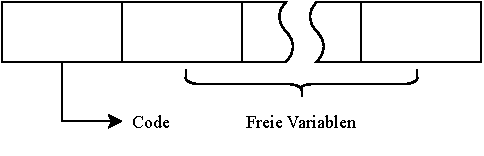
\includegraphics[width=0.8\textwidth]{closure-layout}
  \caption{Aufbau einer Closure}\label{fig:closure}
\end{figure}

%%% Local Variables:
%%% mode: latex
%%% TeX-master: "../Ausarbeitung"
%%% End:


\chapter{Die STG-Sprache}\label{chap:stg}

Die \gls{stg}-Sprache ist eine kleine funktionale Programmiersprache, die eng mit der Semantik der \gls{stg}-Maschine verknüpft ist.
Zudem dient sie als kleiner Sprachkern für Haskell und wird dort im Übersetzungs- und Ausführungsprozess verwendet.

Im Vergleich zu anderen Maschinensprachen fällt auf, dass die \gls{stg}-Sprache eine funktionale Programmiersprache ist.
Anstelle der Beschreibung einzelner Anweisungen oder Instruktionen, die den Zustand der Maschine ändern, werden deklarativ Funktionen beschrieben, deren Zusammenspiel einen Graphen bildet.
Da die Reduktion dieses Graphen der Ausführung der \gls{stg}-Maschine entspricht, gibt es einige Unterschiede zu funktionalen Kern- oder Hochsprachen.
Anstelle viele, einfache Abstraktionen zu schaffen, ist eine genaue Kontrolle über das Verhalten der zugrundeliegenden Maschine gewünscht.

Sowohl die Nähe zur Maschinensemantik als auch die Kontrolle der selben wird bei Betrachtung der verschiedenen Sprachkonstrukte deutlich, die im Folgenden vorgestellt werden.

\begin{figure}
  \centering
  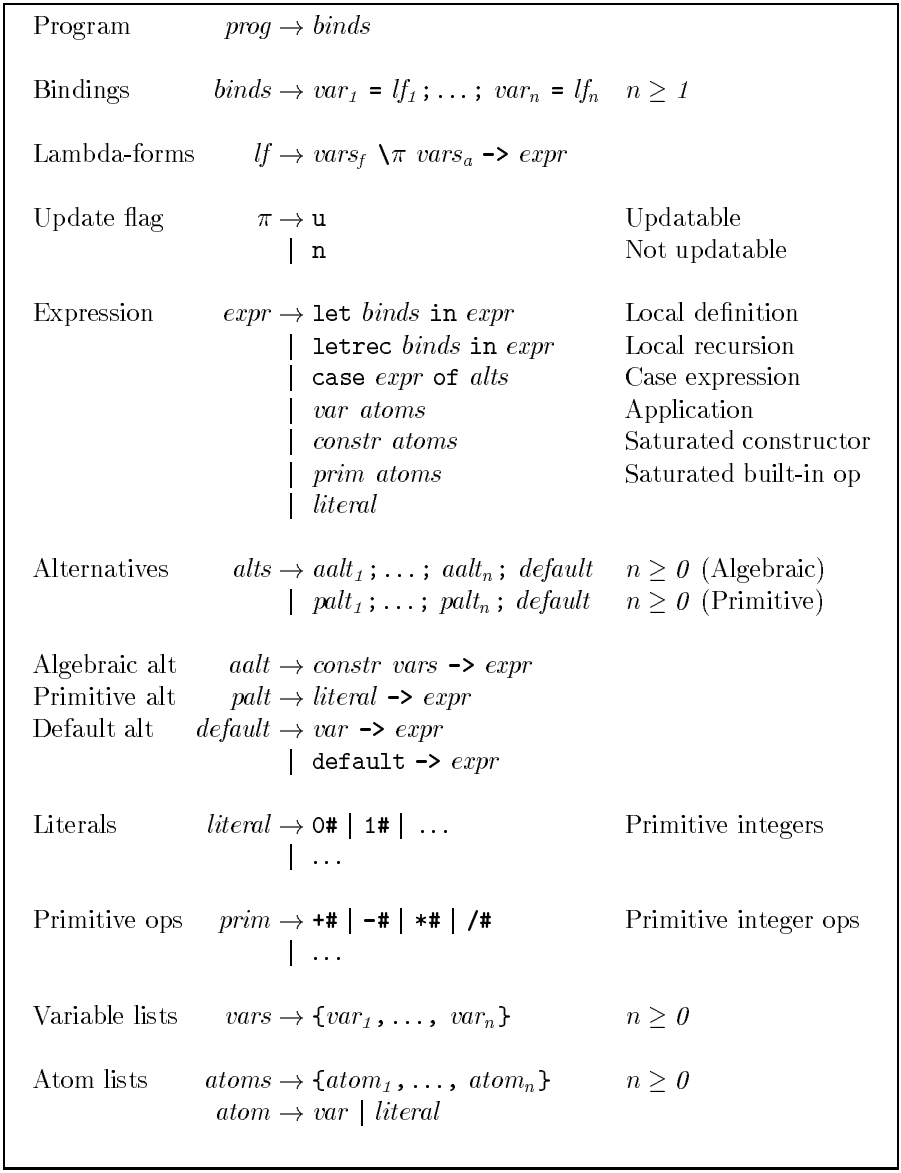
\includegraphics[width=\textwidth]{grammar}
  \caption[Grammatik der STG-Sprache]{Grammatik der STG-Sprache aus \cite{Jones_StockHardwareSTG}}\label{fig:grammar}
\end{figure}

\section{Lambdaformen}

Lambdaformen entsprechen den klassischen Lambdaausdrücken, wie sie aus nahezu allen funktionalen Sprachen bekannt sind.
Zusätzlich zu der Liste an Variablen, an welche die Argumente der anonymen Funktion gebunden werden, und dem Rumpf der Funktion existieren einige Besonderheiten.

Eine zusätzliche Liste an Variablen bei der Definition einer Lambdaform beschreibt die freien Variablen, die beim Erstellen einer Closure gespeichert werden müssen.
Freie Variablen sind Variablen, die in einem Ausdruck verwendet werden, jedoch nicht innerhalb dieses Ausdrucks definiert werden.
Sie entstehen also durch eine umschließende Definition, und müssen als Kontext der Funktion gespeichert werden.
Da dies Speicherplatz benötigt und somit die Ausführung der \gls{stg}-Maschine beeinflusst, werden die freien Variablen explizit angegeben.

Weiterhin fällt auf, dass eine \textit{Update Flag} als Teil der Lambdaform angegeben wird.
Ist diese Flagge auf \texttt{u} gesetzt, wird die Closure im Speicher nach der Auswertung durch den Ergebniswert ersetzt.
Somit wird eine erneute Auswertung unterbunden, die Performance erhöht und keine zusätzliche Berechnungen durchgeführt.
In anderen Fällen ist diese Ersetzung nicht erwünscht.
Wird ein Wert beispielsweise nur einmal berechnet, muss keine Ersetzung stattfinden und der dafür benötigte Aufwand kann eingespart werden.
Ähnlich ist es, wenn die Lambdaform eine Funktion beschreibt, oder der Ausdruck im Rumpf bereits in der \gls{whnf} ist (siehe~\cite[Chap. 4.2]{Jones_StockHardwareSTG}).


\section{Let-Bindungen}

Bindungsausdrücke binden (potentiell mehrere) Lambdaformen an Bezeichner.
Hierbei wird zwischen Bindungsausdrücken mit dem Schlüsselwort \texttt{let} und rekursiven Bindungsausdrücken mit dem Schlüsselwort \texttt{letrec} unterschieden.
Bei Letzterem dürfen die Definitionen des Ausdrucks gegenseitige Querbezüge besitzen.
Bei der ersten Variante ist dies nicht erlaubt.

Als Besonderheit fällt auf, dass lediglich Lambdaformen gebunden werden können.
Dies reflektiert die lazy Evaluation, da so nicht ein Ausdruck selbst oder dessen Wert gebunden wird.

Hinsichtlich der Maschinensemantik beschreiben Bindungsausdrücke immer Speicherallokation.
Für jede gebundene Lambdaform wird eine Closure auf dem Heap angelegt und die Referenz auf diese für die gebundene Variable verwendet.


\section{Anwendungen}

Die \gls{stg}-Maschine kennt Anwendungen von Funktionen, Konstruktoren und primitiven Operationen.
Im Vergleich zu Haskell gilt hier die Einschränkungen, dass die Anwendungen von Konstruktoren und primitiven Operationen immer alle Argumente angegeben sein müssen.
Eine $\eta$-Reduktion, wie sie in Haskell üblich und idiomatisch ist, wird hier nicht durchgeführt.
So ist sichergestellt, dass immer genügend Argumente auf dem Stack liegen, wenn diese Konstrukte ausgewertet werden, wodurch das Erreichen der \gls{whnf} bei der Auswertung von Konstruktoranwendungen und Aufrufe von primitiven Operationen sichergestellt wird.

Als Einschränkungen gilt für diese Ausdrücke, dass die übergebenen Argumente bei einer Anwendung immer atomar sein müssen; lediglich primitive Konstanten und Variablen sind erlaubt.
Dies reduziert die Komplexität der Maschine und erzwingt, dass komplexe Argumente, die ausgewertet werden müssten, explizit als Closure auf dem Heap abgelegt werden, bevor diese als Argument übergeben werden.

Soll eine einzelne Variable als Ausdruck verwendet werden, so muss die Variable als Funktion auf eine leere Parameterliste angewandt werden.
Bei der Auswertung dieses Ausdrucks wird dann zum Rumpf der Closure gesprungen, die an diese Variable gebunden wird.
Diese etwas umständliche Einschränkung bildet syntaktisch direkt das Ausführungsmodell der \gls{stg}-Maschine ab, in der jeder Ausdruck verzögert ausgewertet wird.

\section{Fallunterscheidungen}

Fallunterscheidungen bestehen aus einem untersuchten Ausdruck und einer Reihe an Fällen, die jeweils ein Muster definieren.
Der erste Fall, dessen Muster zu dem untersuchten Ausdruck passt, wird dabei als Ergebnis der Fallunterscheidung ausgewählt.
Ist kein passendes Muster gegeben, so tritt ein Laufzeitfehler auf.

Fallunterscheidungen sind einstufig; sie können nur anhand des äußersten Konstruktors oder einer primitiven Konstante getroffen werden.
Zudem darf ein Standardfall definiert werden, der immer akzeptiert und optional den gesamten Ausdruck an einen Namen bindet.
In der Praxis stellt diese Einschränkung kein Problem dar, da mehrstufige Fallunterscheidungen in einstufige übersetzt werden können~\cite{Wadler_PatternMatching}.

Die Besonderheit in der Semantik von Fallunterscheidungen ist, dass der untersuchte Ausdruck ausgewertet wird.
Somit bieten Fallunterscheidungen die einzige Möglichkeit in der \gls{stg}, die Auswertung eines Ausdrucks zu erzwingen.
Durch die Auswertung des untersuchten Ausdrucks in \gls{whnf} wird sichergestellt, dass der korrekte Fall ausgewählt wird, da nach der Auswertung der passende Konstruktor in ausgewerteter Form vorliegt.
Gleichzeitig wird dabei sichergestellt, dass nicht zu viel ausgewertet wird und die Laziness erhalten bleibt.


\section{Primitive Werte und Arithmetik}

In reinen nicht-strikten Programmiersprachen werden Zahlenwerte und arithmetische Operationen~--~wie alle weiteren Operationen auch~--~als Closures oder Thunks dargestellt, welche die Berechnungen enthalten.
Folglich sind arithmetische Operationen mit hohen Laufzeitkosten verbunden.
Eine einfache Addition zweier Zahlen etwa, erzwingt das Auswerten der Operanden, das Entpacken der ausgewerteten Zahlenwerte, die eigentliche Durchführung der Addition, das Anlegen einer neuen Closure für den Ergebniswert und das anschließende Ablegen des Ergebnisses.

Die \gls{stg} bietet durch primitive Werte eine Möglichkeit, verfügbare Maschinendatentypen und Maschineninstruktionen einer echten Hardware direkt in der abstrakte Maschine abzubilden.
So existiert beispielsweise der primitive Datentyp \texttt{Int\#}, welcher ganzzahlige Maschinenworte darstellt.
Arithmetische Operationen auf diesen primitiven Werten sind beispielsweise als \texttt{+\#}, \texttt{-\#} verfügbar.

Ganz dem Sinne einer Kernelsprache entsprechend, kann ein verzögert ausgewerteter Zahlentyp um diese primitiven Datentypen herum implementiert werden.

\begin{center}
  \texttt{data Int = MkInt Int\#}
\end{center}

Eine solche Definition beschreibt einen algebraischen Datentypen \texttt{Int} mit einem einzelnen Konstruktor \texttt{MkInt}, der eine primitive Ganzzahl akzeptiert.

Arithmetische Operationen, welche die verzögerte Auswertung unterstützen, können auf ähnliche Weise definiert werden, indem Fallunterscheidungen zum Auswerten und Auspacken der Operanden verwendet und das Ergebnis in den Konstruktor des Zahlentyps gepackt wird.
Ein Ausdruck \texttt{(e1 + e2)} in einer höheren Sprache wie Haskell, könnte wie folgt umgeschrieben werden, um verzögerte Auswertung zu unterstützen:

\begin{lstlisting}[language=haskell]
      case e1 of
      MkInt x# -> case e2 of
                  MkInt y# -> case (+# x# y#) of
                              r# -> MkInt r#
\end{lstlisting}

Die Argumente werden genau wie die primitive Addition durch eine Fallunterscheidung ausgewertet.
Das Ergebnis der Addition wird an den Bezeichner \texttt{r\#} gebunden und an den Konstruktor des Zahlentyps übergeben.
Im gezeigten Programmausschnitt wird die Konvention angewandt, Bezeichner für primitive Variablen mit dem Suffix~\texttt{\#} zu versehen, wie es bei den primitiven arithmetischen Operationen ebenfalls der Fall ist.

%%% Local Variables:
%%% mode: latex
%%% TeX-master: "../Ausarbeitung"
%%% End:


\chapter{Implementierung}\label{chap:implementierung}





%%% Local Variables:
%%% mode: latex
%%% TeX-master: "../Ausarbeitung"
%%% End:


\chapter{Ergebnisse}\label{chap:ergebnisse}

Mit den Regeln aus Kapitel~\ref{chap:implementierung} und den vorgestellten Sprachkonstrukten aus Kapitel~\ref{chap:stg} ist es nun möglich, in der \gls{stg}-Sprache geschriebene, nicht-strikte Programme auszuwerten.
Die Ausführung erfolgt dabei entsprechend der Spezifikation, ermöglicht die Integration von primitiven Java-Operationen und arbeitet korrekt auf allen unterstützten Werten von primitiven Zahlen, über einfache Datentypen bis hin zu Funktionen und verzögert ausgewerteten oder sogar endlosen Datenstrukturen.

Die vollständige Implementierung in Java ist auf GitHub verfügbar.\footnote{\url{https://github.com/Niklas-Deworetzki/java-stg}}
Im selben Projekt befinden sich neben den verschiedenen Quelldateien auch eine Prelude, die vor der Ausführung von \gls{stg}-Programmen geladen werden kann, um einige häufig verwendete Funktionen bereitzustellen.

Das Projekt erfüllt dabei die Ansprüche und Ziele, die zu Beginn gesetzt wurden und präsentiert eine einfache aber funktionstüchtige Implementierung einer virtuellen \gls{stg}-Maschine.
Zusätzlich werden durch die Prelude die Eigenschaften der \gls{stg}-Sprache als Kernsprache hervorgehoben und exemplarisch gezeigt, wie höhere Abstraktionsebenen in die maschinennahe Sprache eingeführt werden können.
Das Hauptziel, die Semantik der \gls{stg}-Maschine korrekt abzubilden wurde erreicht.
Darüber hinaus werden einige der Erweiterungen, die von der \gls{stg} vorgestellt werden, implementiert.
Neben der \textit{spineless} Darstellung eines Programms, die durch Verwendung der \gls{stg} \enquote{geschenkt} ist, wird auch die \textit{tagless} Darstellung implementiert.
Die verschiedenen Maschinenzustände werden nicht durch explizite Tags unterschieden.
Stattdessen werden sie durch den Aufruf einer Methode dynamisch zur Laufzeit ausgewählt.
Zudem werden auch Optimierungen, wie etwa das Aktualisieren von ausgewerteten Closures, unterstützt.

\section{Wichtige Erweiterungen}

Obwohl die Kernfunktionalität der \gls{stg} implementiert ist und auch die besonderen Eigenschaften der Maschine unterstützt werden, existieren einige Erweiterungen und diskutierte Optimierungen aus~\cite{Jones_StockHardwareSTG}, die nicht implementiert sind.

Viele der möglichen Erweiterungen, die sich in die \gls{stg}-Maschine einbauen lassen, sind in erster Linie dazu gedacht, die Programmierung zu erleichtern oder den produktiven Betrieb zu ermöglichen.
So kann beispielsweise ein Foreign Function Interface bereitgestellt werden, um mit existierenden Bibliotheken anderer Programmiersprachen zu interagieren~\cite{Jones_TacklingAwkwardSquad}.
Die Implementierung dieser Schnittstelle ist dabei ähnlich wie die Integration eingebauter, primitiver Funktionen.

Eine weitere hilfreiche Erweiterung baut auf das Aktualisieren von Closures auf.
Wird eine Closure nachdem sie betreten wurde, aber bevor sie vollständig ausgewertet wird, durch einen speziellen Wert ersetzt, lassen sich Fehler zur Laufzeit entdecken.
Ein sogenanntes \textit{Black Hole} lässt sich für eine betretene Closure einsetzen, mit der Eigenschaft, dass das Betreten eines solchen Loches einen Fehler wirft.
Der Fehlerfall tritt nur dann auf, wenn während der Auswertung einer Closure, die selbe Closure erneut betreten wird.
Das bedeutet, dass ein Wert von sich selbst abhängig ist und nicht berechnet werden kann~\cite{Jones_StockHardwareSTG}.

Anstelle eines Black Holes, können aber auch andere besondere Darstellungen für Closures eingesetzt werden.
Beispielsweise ist es möglich, betretene Closures durch Synchronisierungsblöcke zu ersetzen.
Dadurch können mehrere Closures gleichzeitig betreten und in unterschiedlichen Threads ausgewertet werden.
Ist die Auswertung abgeschlossen sorgen die Synchronisierungsblöcke dafür, dass die verschiedenen Threads wieder zusammengeführt werden.
Auf diese Weise kann unsichtbar für einen Nutzer Parallelisierung implementiert werden~\cite{Jones_StockHardwareSTG}.

Die Wohl wichtigste Erweiterung, die zunächst notwendig ist, um die produktive Verwendung der Implementierung überhaupt in Betracht ziehen zu können, ist die Implementierung eines Garbage Collectors.
Die Sprachsemantik definiert nur ein Konstrukt für die Speicherallokation.
Eine kontrollierte Speicherfreigabe ist nicht vorgesehen.
Stattdessen werden einige Algorithmen präsentiert, die automatisch ungenutzte Closures auf dem Heap erkennen und freigeben können~\cite{Jones_StockHardwareSTG}.
Wird ein solcher Algorithmus angestoßen, wenn nicht mehr genügend Speicher verfügbar ist oder läuft er dauerhaft im Hintergrund, ist es möglich, nicht benötigten Speicher freizugeben und auf dem Heap lediglich Closures zu halten, die für die Auswertung relevant sind.

\section{Schwachstellen der Implementierung}

Auch wenn sie entsprechend der Beschreibung arbeitet, existieren einige Schwachstellen in der vorgestellten Implementierung.
Diese Beziehen sich hauptsächlich auf die Ausführung und die Nutzerfreundlichkeit der Maschine.

Ein Beispiel hierfür ist der Abschluss der Ausführung.
Die Maschine selbst sieht keinen Endzustand vor, in dem die Ausführung abgeschlossen ist und der von außerhalb eindeutig als solcher Erkannt werden kann.
Stattdessen wird~--~wie in Abschnitt~\ref{sec:runtime} dargestellt~--~erkannt, wenn beim Ersetzen einer Closure auf den leeren Update-Stack zugegriffen wird.
Liegt in einem solchen Fall ein \textit{Return Integer} oder \textit{Return Constructor}-Zustand vor, wird der von diesen zurückgegebene Wert als Ergebnis der Maschine angezeigt.
Dabei wird lediglich die Zahl als Text formatiert oder der Name des Konstruktors ausgegeben.
Komponenten von Datenstrukturen liegen lediglich als Adresse auf dem Heap und womöglich unausgewertet dem Konstruktor vor.
Eine komplexere Ausgabe ist also nicht ohne Weiteres möglich.

Auch vor dem Erreichen eines Programmendes können nutzerunfreundliche Eigenschaften der Implementierung beobachtet werden.
Liegt in einem ausgeführten \gls{stg}-Programm ein Fehler vor, so ist das Verhalten der Maschine oftmals unerwartet (wenn auch Korrekt bezüglich der Maschinensemantik).
Fehler werden an scheinbar willkürlichen Stellen bekannt und durch die verzögerte Auswertung teilweise auch erst in späteren Programmabschnitten relevant.
Ohne einen Debugger und eine intuitive Darstellung von komplexen Werten wird das Debugging oft zu einem Ratespiel.

Der Hauptnutzen bei der Implementierung liegt wohl im akademischen Wert und in der gesammelten Erfahrung.
Doch auch hier werden einige Kapitel aus~\cite{Jones_StockHardwareSTG} ausgelassen.
In einer Sprache, die mehr Kontrolle über Speicherlayout und Speicherallokation bietet, wäre es möglich, Diskussionen über die Darstellung und das Speicherlayout von Closures sowie die Speicherverwaltung mit einem Garbage Collector nachzuvollziehen.
Eine vollständige Implementierung all dieser Aspekte sprengt jedoch den Rahmen (und auch den Fokus) dieser Veranstaltung bei Weitem.


\section{Vergleich mit anderen Implementierungen}

Letztlich soll die entstandene Implementierung im Vergleich zu bereits existierendem Material zur \gls{stg}-Maschine eingeordnet werden.
Viele weitere Implementierungen der \gls{stg}-Maschine sind nicht bekannt.
Jedoch wird sie gerade im Kontext von Haskell benutzt und dementsprechend auch Weiterentwickelt.
Hier ist als größte Erweiterung ein anderer Ansatz bei der Übergabe von Funktionsargumenten zu nennen, wodurch gerade bei Funktionen höherer Ordnung für die häufigsten Anwendungsfälle die Performance verbessert wird~\cite{PeytonJones_FastCurry}.

Als andere Implementierung der \gls{stg}-Maschine existiert das Projekt \textit{STGi}~\cite{Luposchainsky_StgInterpreter}.
Geschrieben in Haskell steht dieser Interpreter für die \gls{stg}-Sprache als Lehrbeispiel zur Verfügung.
Mit einer textuellen Darstellung von Werten, Zuständen und Zustandsübergängen sowie implementierten Erweiterungen wie Black Holes, Garbage Collection und der Semantik aus~\cite{PeytonJones_FastCurry}, liegt der Fokus dieser Implementierung jedoch darauf, die Ausführung interaktiv zu begleiten.
Die Arbeit, welche die \gls{stg} bei der Übersetzung in imperative Anweisungen betreibt, wird bei der Implementierung in Haskell nicht deutlich.

Die wohl wichtigste \gls{stg}-Implementierung befindet sich ebenfalls in der Domäne von Haskell.
Der sogenannte GHC Haskell Compiler verwendet intern die \gls{stg}, um Maschinencode entweder nativ oder mittels LLVM zu erzeugen.
Dabei bietet diese Implementierung nicht nur Unterstützung für viele Erweiterungen, Optimierungen, Tooling und Profiling, sondern stellt auch eine produktionsreife Ausführungsumgebung für Haskell bereit.
Als de facto Standard für Haskell, ist hier die wohl ausgereifteste Implementierung zu finden.
Geschrieben in Haskell, über Jahre gewachsen und mit Unterstützung für Optimierungen ist sie jedoch nicht als Lehrbeispiel geeignet.

Zusammenfassend ist dieses Projekt eher als Lern- und Spielzeugprojekt zu einzuordnen.
Der Hauptzweck der Implementierung ist es, innerhalb des Kurses \textit{CS5341~--~Kernel-Architekturen in Programmiersprachen} Erfahrungen  zu sammeln, neue Berechnungsmodelle zu untersuchen und den eigenen Horizont zu erweitern.

%%% Local Variables:
%%% mode: latex
%%% TeX-master: "../Ausarbeitung"
%%% End:



%==============================================================================

% end matter
\pagenumbering{Roman}
\addtocounter{savepage}{1}
\setcounter{page}{\value{savepage}}

% list of tables and figures
\listoffigures
\lstlistoflistings

% Bibliography
\printbibliography[heading=bibintoc, title=Literaturverzeichnis]{}

% Appendices
\appendix

\end{document}

%%% Local Variables:
%%% mode: latex
%%% TeX-master: t
%%% End:
